\documentclass{article}

\usepackage[a4paper, top=1in, bottom=1in, left=0.7in, right=1.2in]{geometry}
\usepackage{multicol}
\usepackage{tikz}
\usetikzlibrary{arrows}
\usepackage{graphicx}
\usepackage{amsmath}
\usepackage{amssymb}
\usepackage[table]{xcolor}

\definecolor{obsidianDarkGray}{HTML}{131313} % A common dark gray for backgrounds
\definecolor{obsidianLightGray}{HTML}{CCCCCC} % A common light gray for text

\pagecolor{obsidianDarkGray} % Set page background to dark gray
\color{obsidianLightGray} % Set default text color to light gray

% \pagecolor{black}
% \color{white}

\title{Algoritmi v bioinformatiki - 2. Domača naloga}
\author{Jan Panjan}
\date{\today}

\begin{document}

\maketitle

\newpage

\begin{enumerate}
	\item  \textit{Dano imamo naslednje zaporedje izidov metov kovanca}

		$$
		V = CCCGCGGCCGC
		$$

		\textit{pri čemer $C$ označuje, da je bil izid meta cifra, $G$ pa da je bil izid meta grb.
		Za mete imamo na voljo 3 kovance, $A$, $B$ in $C$, veljajo naslednje verjetnosti:}

		\begin{tabular}{cc||c|c|c|}
			\multicolumn{1}{c}{\textit{Prehod:}} & \%  & A & B & C\tabularnewline
			\cline{2-5}
										& A & 40 & 30 & 30 \tabularnewline
										\cline{2-5}
										& B & 30 & 40 & 30\tabularnewline
										\cline{2-5}
										& C & 30 & 30 & 40 \tabularnewline
		\end{tabular}$\,\,\,\,\,\,\,\,\,\,\,\,\,\,\,\,\,\,\,\,$%
		\begin{tabular}{cc||c|c|}
			\multicolumn{1}{c}{\textit{Izpis:}} & \% & C & G\tabularnewline
			\cline{2-4}
									   & A & 75 & 25\tabularnewline
									   \cline{2-4}
									   & B & 80 & 20\tabularnewline
									   \cline{2-4}
									   & C & 20 & 80\tabularnewline
		\end{tabular}

		\textit{Katera od možnosti je najbolj verjetna?}

			\begin{enumerate}
				\item \textit{za vse mete smo uporabili kovanec A}
				\item \textit{za vse mete smo uporabili kovanec C}
				\item \textit{za vse mete smo uporabili kovanec B}
				\item \textit{$\Pi$ = AAACBCCBBCA}
			\end{enumerate}

			\textit{Odgovor ustrezno utemeljite.}

			-----------------------------------------------------------------------------------------------------------------------------------

			\textbf{Za vse mete smo uporabili kovanec A}

			\begin{center}
				\begin{tabular}{c||l}
					$(0.75)^7$ & 7-krat vržemo C z verjetnostjo $0.75$ \\
					\hline
					$(0.25)^2$ & 7-krat vržemo G z verjetnostjo $0.75$ \\
					\hline
					$(0.4)^{10}$ & 10-krat ne zamenjamo kovanca $A$ z verjetnostjo $0.4$
				\end{tabular}

				$$
				p(A) = (0.75)^7 \cdot (0.25)^4 \cdot (0.4)^{10} = 0.00209
				$$
			\end{center}

			\textbf{Za vse mete smo uporabili kovanec B}

			\begin{center}
				\begin{tabular}{c||l}
					$(0.8)^7$ & 7-krat vržemo C z verjetnostjo $0.8$ \\
					\hline
					$(0.2)^2$ & 7-krat vržemo G z verjetnostjo $0.2$ \\
					\hline
					$(0.4)^{10}$ & 10-krat ne zamenjamo kovanca $B$ z verjetnostjo $0.4$
				\end{tabular}

				$$
				p(B) = (0.8)^7 \cdot (0.2)^4 \cdot (0.4)^{10} = 0.00134
				$$
			\end{center}

			\textbf{Za vse mete smo uporabili kovanec C}

			\begin{center}
				\begin{tabular}{c||l}
					$(0.2)^7$ & 7-krat vržemo C z verjetnostjo $0.8$ \\
					\hline
					$(0.8)^2$ & 7-krat vržemo G z verjetnostjo $0.2$ \\
					\hline
					$(0.4)^{10}$ & 10-krat ne zamenjamo kovanca $C$ z verjetnostjo $0.4$
				\end{tabular}

				$$
				p(C) = (0.2)^7 \cdot (0.8)^4 \cdot (0.4)^{10} = 0.0000209
				$$
			\end{center}

			\textbf{$\Pi$ = AAACBCCBBCA}

			\begin{center}
				\begin{tabular}{c||l}
					$(0.3)^6$ & 6-krat ostanemo v istem kovancu (vsi kovanci imajo enake verjetnosti) \\
					\hline
					$(0.4)^4$ & 4-krat zamenjamo kovanec (tudi tu imajo enako verjetnosti) \\
					\hline
					$(0.75)^4$ & 4-krat vržemo kovanec $A$, vsakič vržemo cifro z verjetnostjo $0.75$ \\
					\hline
					$(0.8)^3$ & 3-krat vržemo kovanec $B$, vsakič vržemo cifro z verjetnostjo $0.8$ \\
					\hline
					$(0.8)^4$ & 4-krat vržemo kovanec $C$, vsakič vržemo grb z verjetnostjo $0.8$
				\end{tabular}

				$$
				p(\Pi) = (0.3)^6 \cdot (0.4)^4 \cdot (0.75)^4 \cdot (0.8)^3 \cdot (0.8)^4 = 0.00000124
				$$
			\end{center}

			-----------------------------------------------------------------------------------------------------------------------------------

		\textbf{Rešitev:} Najbolj verjetna je možnost z največjo verjetnostjo. To je možnost (a)
		z verjetnostjo $0.00209$.

		\newpage

	\item \textit{Dani imamo zaporedji $s=GAGTACA$ in $t=TGATTACA$ ter vrednostno funkcijo s parametroma
		$\mu = 4, \sigma = 2$ in nagrado za ujemanje 2.}

		\begin{enumerate}
			\item \textit{Z uporabo Needleman-Wunsch-evega algoritma za globalno poravnavo smo dobili
				naslednjo tabelo:}

				\begin{center}
					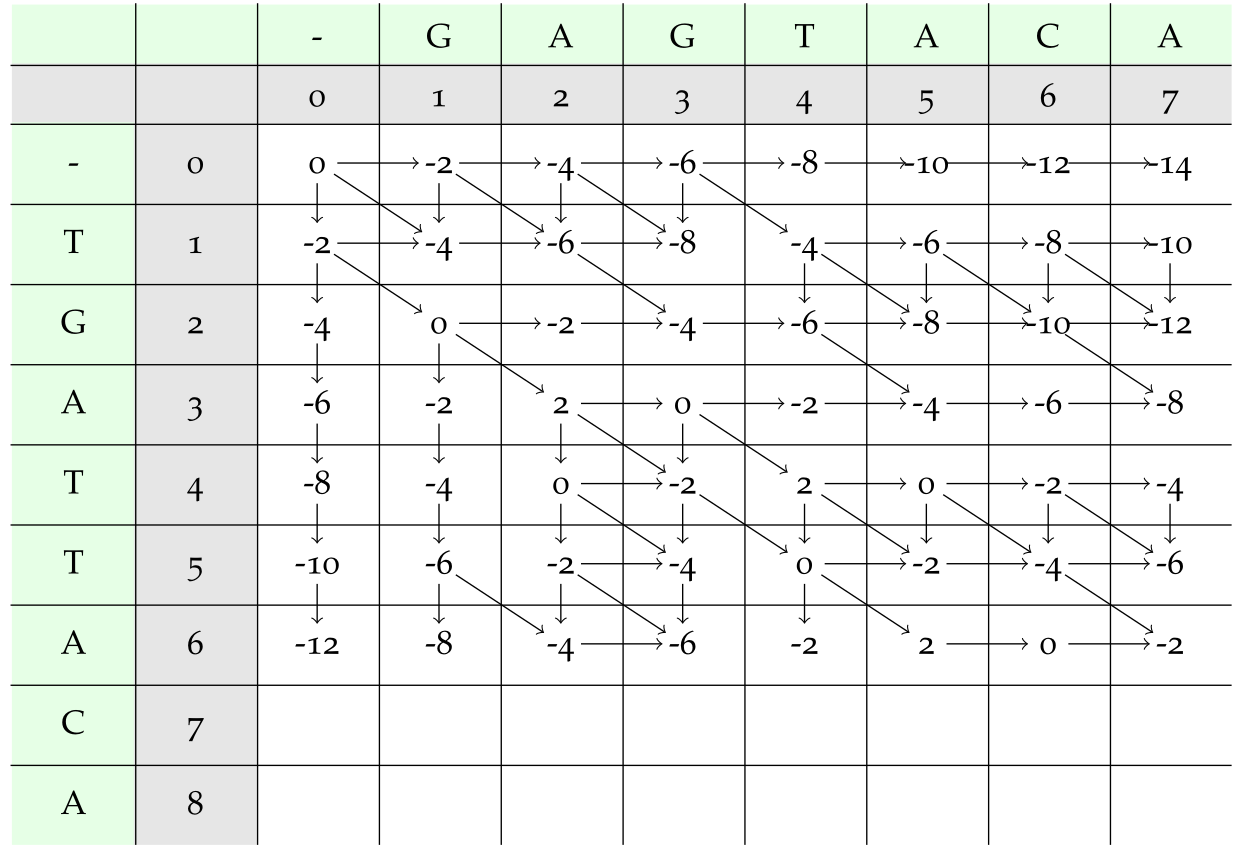
\includegraphics[scale=0.17]{NW-tabela.png}
				\end{center}

				\textit{Dopolnite tabelo tako, da poračunate vrednosti (in ustrezne puščice) za zadnji dve vrstici.}

				\begin{center}
					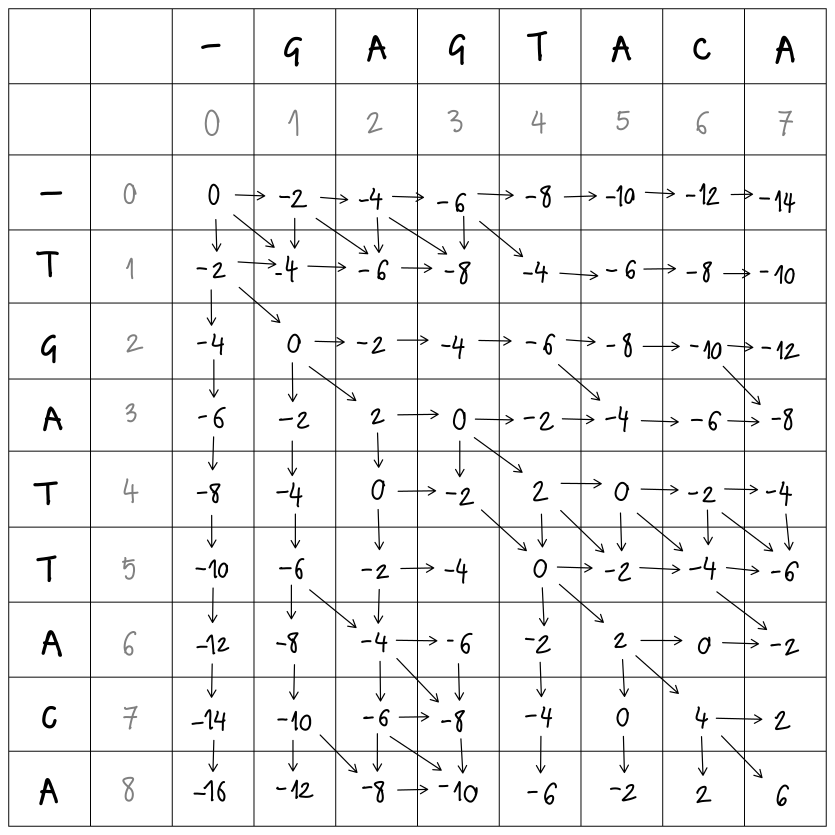
\includegraphics[scale=0.21]{matrika-complete-1.png}
				\end{center}

			\item \textit{Koliko optimalnih globalnih poravnav dobite? Izpišite vse rešitve.}

			------------------------------------------------------------------------------------------------------------------------------

				Dobim dve optimalni globalni poravnavi. Mesto vrzeli se spremeni in sicer iz mesta 4 na mesto 3 (in obratno):

				\begin{multicols}{2}
					\begin{tabular}{c||c|c|c|c|c|c|c|c|c}
						s & - & G & A & G & \textcolor{red}{T} & \textcolor{red}{-} & A & C & A \\
						\hline
						t & T & G & A & - & \textcolor{red}{T} & \textcolor{red}{T} & A & C & A
					\end{tabular}

					\begin{tabular}{c||c|c|c|c|c|c|c|c|c}
						s & - & G & A & G & \textcolor{red}{-} & \textcolor{red}{T} & A & C & A \\
						\hline
						t & T & G & A & - & \textcolor{red}{T} & \textcolor{red}{T} & A & C & A
					\end{tabular}
				\end{multicols}

				Z matrikami to izgleda tako:

				\begin{multicols}{2}
					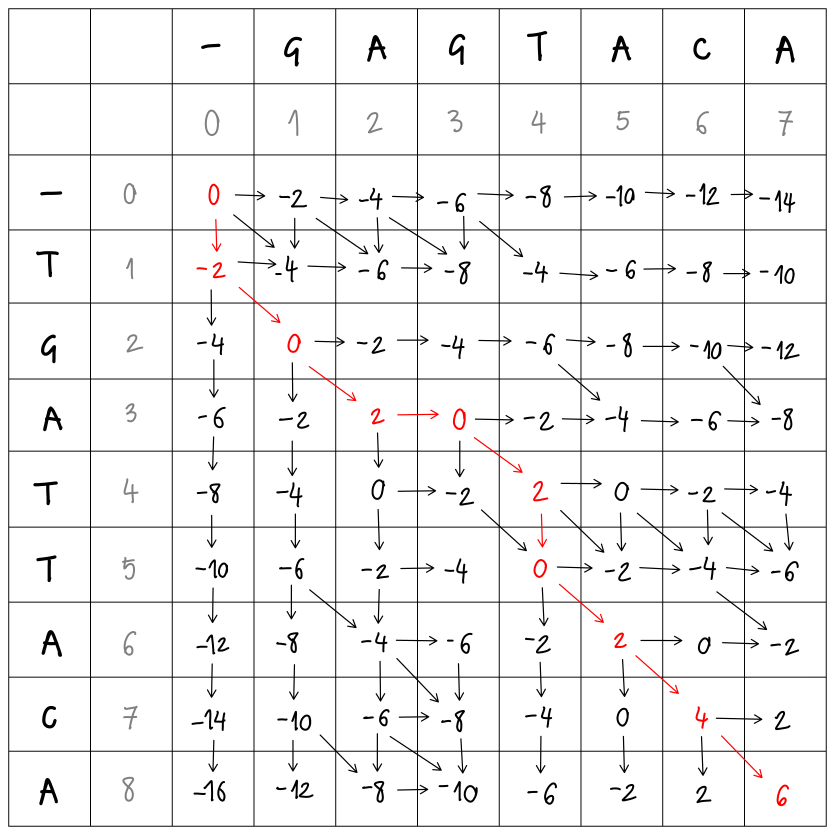
\includegraphics[scale=0.23]{matrika-complete-2}

					\columnbreak

					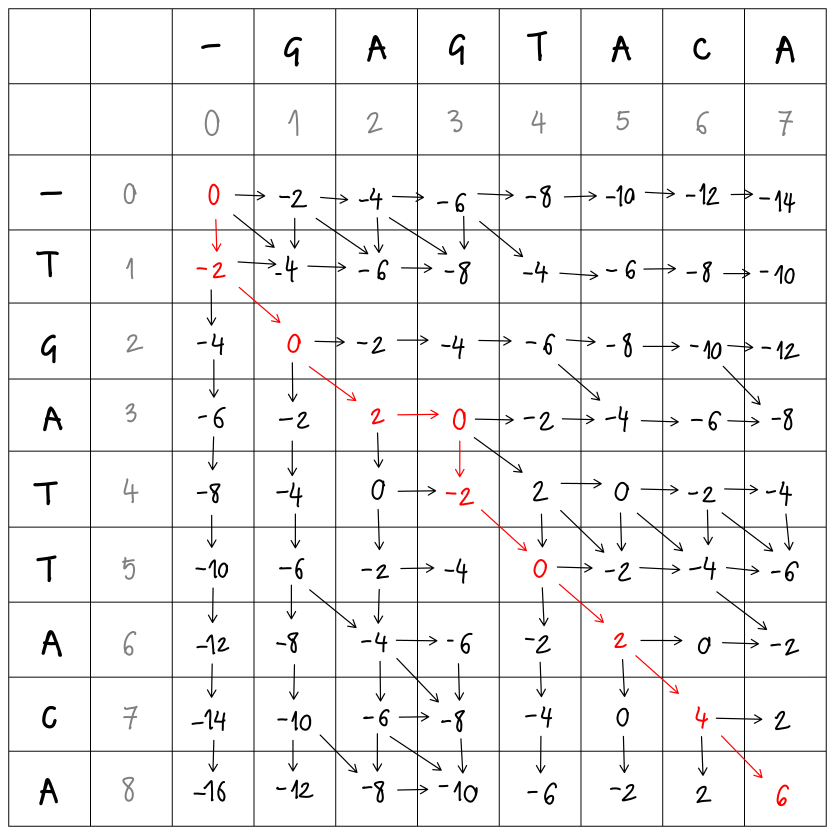
\includegraphics[scale=0.23]{matrika-complete-3}
				\end{multicols}
		\end{enumerate}

		\newpage

	\item \textit{Dano imamo naslednjo matriko izražanja:}

		\begin{center}
			\begin{tabular}{c||c|c|c|c|c|c|}
				& $T_1$ & $T_2$ & $T_3$ & $T_4$ & $T_5$ & $T_6$ \\
				\hline
				\hline
				$g_1$ & 2 & 2 & 6 & 2 & 3 & 4 \\
				\hline
				$g_2$ & 3 & 7 & 3 & 1 & 9 & 3 \\
				\hline
				$g_3$ & 2 & 2 & 7 & 2 & 6 & 3 \\
				\hline
				$g_4$ & 3 & 2 & 3 & 2 & 1 & 3 \\
				\hline
				$g_5$ & 2 & 1 & 5 & 1 & 0 & 4 \\
				\hline
				$g_6$ & 3 & 5 & 5 & 8 & 2 & 3 \\
				\hline
				$g_7$ & 1 & 3 & 1 & 5 & 4 & 2 \\
				\hline
				$g_8$ & 5 & 4 & 2 & 4 & 7 & 5
			\end{tabular}
		\end{center}

		\textit{Določite gruče z uporabo metode voditeljev, če je začetna množica voditeljev
		enaka $X = \{g_1, g_5, g_6\}$.}

		Vsak gen lahko obravnavamo kot vektor $g_i = (T_1, \dots, T_6)$.

		-----------------------------------------------------------------------------------------------------------------------------------

		\begin{center}
			\paragraph{Prva iteracija}
		\end{center}

		\paragraph{Prvi korak} Najprej je potrebno izračunati razdalje med geni.
		(Evklidska) razdalja med vsakim genom je definirana kot:

		\begin{equation}
			d(g_i, g_j) = \sqrt{ \left(T_{i}^{(1)} - T_{j}^{(1)} \right)^2 + \dots + \left(T_{i}^{(6)} - T_{j}^{(6)} \right)^2 } \quad ; \quad 1 \leq i,j \leq 8
		\end{equation}

		Primer za prvi gen:

		$$
		d(g_1, g_1) = \sqrt{ (2-2)^2 + (2-2)^2 + (6-6)^2 + (2-2)^2 + (3-3)^2 + (4-4)^2 } = 0
		$$

		Očitno je razdalja med istim genom 0, kar pravi tudi prva lastnost metrike: $d(x,y) = 0 \iff x = y$.

		Ko poračunamo vse, dobimo matriko razdalj. Potrebujemo razdalje samo do voditeljev:

		\begin{center}
			\begin{tabular}{c||c|c|c|}
				& $d(g_1, g_i)$ & $d(g_5, g_i)$ & $d(g_6, g_i)$ \\
				\hline
				\hline
				$g_1$ & 0 & 18.166 & 17.493\\
				\hline
				$g_2$ & 8.544 & 11.091 & 10.296\\
				\hline
				$g_3$ & 3.317 & 6.557 & 8.124\\
				\hline
				$g_4$ & 3.873 & 3.000 & 7.071\\
				\hline
				$g_5$ & 18.166 & 0 & 10.198\\
				\hline
				$g_6$ & 17.493 & 10.198 & 0\\
				\hline
				$g_7$ & 5.657 & 7.071 & 5.568\\
				\hline
				$g_8$ & 7.071 & 9.274 & 7.681\\
			\end{tabular}
		\end{center}

		\paragraph{Drugi korak} Za vsak gen izberemo najkrajšo razdaljo med njim in voditeljem.

		\begin{center}
			\begin{tabular}{c||c|c|c|}
				& $d(g_1, g_i)$ & $d(g_5, g_i)$ & $d(g_6, g_i)$ \\
				\hline
				\hline
				$g_1$ & \textcolor{red}{0} & 18.166 & 17.493\\
				\hline
				$g_2$ & \textcolor{red}{8.544} & 11.091 & 10.296\\
				\hline
				$g_3$ & \textcolor{red}{3.317} & 6.557 & 8.124\\
				\hline
				$g_4$ & 3.873 & \textcolor{red}{3.000} & 7.071\\
				\hline
				$g_5$ & 18.166 & \textcolor{red}{0} & 10.198\\
				\hline
				$g_6$ & 17.493 & 10.198 & \textcolor{red}{0}\\
				\hline
				$g_7$ & 5.657 & 7.071 & \textcolor{red}{5.568}\\
				\hline
				$g_8$ & \textcolor{red}{7.071} & 9.274 & 7.681\\
			\end{tabular}
		\end{center}

		\paragraph{Tretji korak} Iz vsakega stolpca odčitamo nove voditelje (vrednosti označene z
		rdečo), katere označimo s $C_i, i \in\mathbb{N}$, in sicer:

		\begin{align*}
			C_1 &= \left\{ g_1, g_2, g_3, g_8 \right\} \\
			C_2 &= \left\{ g_4, g_5 \right\} \\
			C_3 &= \left\{ g_6, g_7 \right\}
		\end{align*}

		\paragraph{Četrti korak} Za gručo $C_i$ z $n$ geni $\left\{ g_1, \dots, g_{k} \ | \ 1 \leq k \leq 8 \right\}$,
		izračunamo nov vektor vrednosti $v_i = \left( v_{i1}, \dots, v_{in} \right)$ z enačbo:

		\begin{equation}
			v_{i} = \frac{ 1 }{ n} \sum_{j=1}^{n} g_{k}
		\end{equation}

		Nove vrednosti so torej aritmetična sredina vseh genov v gruči:

		\begin{align*}
			v_1 &= ( 3,   3.75, 4.5, 2.25, 6.25, 3.75 ) \\
			v_2 &= ( 2.5, 1.5,  4,   1.5,  0.5,  3.5 ) \\
			v_3 &= ( 2,   4,    3.5, 6.5,  3,    2.5 )
		\end{align*}

		Zdaj ponovimo korake dokler ne dosežemo \textbf{konvergence}:

		\begin{itemize}
			\item ko se gruče med iteracijama ne spremenijo
			\item ko postanejo razlike med radaljami gruč manjše od neke vnaprej določene vrednosti.
		\end{itemize}

		-----------------------------------------------------------------------------------------------------------------------------------

		\begin{center}
			\paragraph{Druga iteracija}
		\end{center}

		\paragraph{Prvi + drugi korak}

		\begin{center}
			\begin{tabular}{c||c|c|c|}
				& $d(v_1, g_i)$ & $d(v_2, g_i)$ & $d(v_3, g_i)$ \\
				\hline
				\hline
				$g_1$ & \textcolor{red}{3.808} & 3.354 & 5.723\\
				\hline
				$g_2$ & \textcolor{red}{4.743} & 10.209 & 8.761\\
				\hline
				$g_3$ & \textcolor{red}{3.317} & 6.344 & 6.764\\
				\hline
				$g_4$ & 5.788 & \textcolor{red}{1.500} & 5.454\\
				\hline
				$g_5$ & 7.036 & \textcolor{red}{1.500} & 7.263\\
				\hline
				$g_6$ & 7.314 & 7.632 & \textcolor{red}{2.784}\\
				\hline
				$g_7$ & 5.148 & 5.958 & \textcolor{red}{2.784}\\
				\hline
				$g_8$ & \textcolor{red}{3.937} & 8.185 & 6.305\\
			\end{tabular}
		\end{center}

		\paragraph{Tretji korak}

		\begin{align*}
			C_4 &= \left\{ g_1, g_2, g_3, g_8 \right\} \\
			C_5 &= \left\{ g_4, g_5 \right\} \\
			C_6 &= \left\{ g_6, g_7 \right\}
		\end{align*}

		Ker so gruče enake kot v prejšnji iteraciji, lahko postopek tu končamo\dots

		-----------------------------------------------------------------------------------------------------------------------------------

		\textbf{Rešitev:} gruče določene z metodo voditeljev s $k=3$ za dano matriko
		izražanja so

		\begin{align*}
				&\left\{ g_1, g_2, g_3, g_8 \right\}  \\
				&\left\{ g_4, g_5 \right\}  \\
				&\left\{ g_6, g_7 \right\}
		\end{align*}

		\newpage

	\item \textit{Izračunajte drevo hierarhičnega gručenja z uporabo algoritma UPGMA.}

		Naj bo množica vseh genov $G = \{g_1, \dots, g_8 \}$.
		Osnova za algoritem UPGMA je matrika razdalj genov, za katero uporabimo sledečo enačbo

		\begin{equation}
			d_{\text{avg}}(C, C^*) = \frac{ 1 }{ |C| |C^*| } \sum_{x\in C, y\in C^*} d(x,y)
		\end{equation}

		kjer sta $C$ in $C^*$ dve gruči (na začetku so to geni). $d$ je ista kot v (1).

		\begin{center}
			\begin{tabular}{c||c|c|c|c|c|c|c|c|}
				& $g_1$ & $g_2$ & $g_3$ & $g_4$ & $g_5$ & $g_6$ & $g_7$ & $g_8$ \\
				\hline
				\hline
				$g_1$ & 0     & 8.544 & 3.317 & 3.873 & 3.464 & 7.000 & 5.657 & 7.071 \\
				\hline
				$g_2$ &       & 0     & 8.124 & 10.198 & 11.091 & 10.296 & 10.677 & 8.602 \\
				\hline
				$g_3$ &       &       & 0     & 6.325 & 6.557  & 8.124  & 6.403 & 7.000 \\
				\hline
				$g_4$ &       &       &       & 0     & 3.000  & 7.071  & 5.099 & 6.403 \\
				\hline
				$g_5$ &       &       &       &       & 0      & 10.198 & 7.071 & 9.274 \\
				\hline
				$g_6$ &       &       &       &       &        & 0      & 5.568 & 7.681 \\
				\hline
				$g_7$ &       &       &       &       &        &        & 0     & 5.916 \\
				\hline
				$g_8$ &       &       &       &       &        &        &        & 0     \\
			\end{tabular}
		\end{center}

		Gručenje deluje tako, da vsako iteracijo izberemo najbližja gena in ju združimo
		v gručo. Na začetku je vsak gen v svoji gruči, do konca postopka pa ustvarimo eno
		celovito gručo, ki bo vsebovala vse gene.

		-----------------------------------------------------------------------------------------------------------------------------------

		\begin{center}
			\paragraph{Prva iteracija}
		\end{center}

		\paragraph{Prvi korak} Izberemo najmanjšo vrednost med razdaljami.

		\begin{center}
			\begin{tabular}{c||c|c|c|c|c|c|c|c|}
				& $g_1$ & $g_2$ & $g_3$ & $g_4$ & $g_5$ & $g_6$ & $g_7$ & $g_8$ \\
				\hline
				\hline
				$g_1$ & 0     & 8.544 & 3.317 & 3.873 & 3.464 & 7.000 & 5.657 & 7.071 \\
				\hline
				$g_2$ &       & 0     & 8.124 & 10.198 & 11.091 & 10.296 & 10.677 & 8.602 \\
				\hline
				$g_3$ &       &       & 0     & 6.325 & 6.557  & 8.124  & 6.403 & 7.000 \\
				\hline
				$g_4$ &       &       &       & 0     & \textcolor{red}{3.000}  & 7.071  & 5.099 & 6.403 \\
				\hline
				$g_5$ &       &       &       &       & 0      & 10.198 & 7.071 & 9.274 \\
				\hline
				$g_6$ &       &       &       &       &        & 0      & 5.568 & 7.681 \\
				\hline
				$g_7$ &       &       &       &       &        &        & 0     & 5.916 \\
				\hline
				$g_8$ &       &       &       &       &        &        &        & 0     \\
			\end{tabular}
		\end{center}

		\paragraph{Drugi korak} Dodamo gena v gručo $C_1$, torej $C_1 = \{g_4, g_5\}$ in poračunamo
		novi vektor $v_1$, ki bo predstavljal novo gručo v matriki razdalj (tako kot prej uporabimo
		aritmetično sredino komponent vrednosti iz matrike izražanja):

		$$
		v_1 = (2.5, \ 1.5, \ 4, \ 1.5, \ 0.5, \ 3.5)
		$$

		\paragraph{Tretji korak} Gena v gruči združimo, tako da je $G = \{g_1, \dots, C_1, \dots, g_8\}$.
		Izračunamo razdaljo gruče ($C_1$) do vseh ostalih gruč s pomočjo enačbe (3).

		\begin{center}
			\begin{tabular}{c||c|c|c|c|c|c|c|}
				& $g_1$ & $g_2$ & $g_3$ & $C_1$ & $g_6$ & $g_7$ & $g_8$ \\
				\hline
				\hline
				$g_1$ & 0     & 8.544 & 3.317 & 3.669 & 7.000 & 5.657 & 7.071 \\
				\hline
				$g_2$ &       & 0     & 8.124 & 10.645& 10.296 & 10.677 & 8.602 \\
				\hline
				$g_3$ &       &       & 0     & 6.441 & 8.124  & 6.403 & 7.000 \\
				\hline
				$C_1$ &       &       &       & 0     & 8.635  & 6.085 & 7.839 \\
				\hline
				$g_6$ &       &       &       &       & 0      & 5.568 & 7.681 \\
				\hline
				$g_7$ &       &       &       &       &        & 0     & 5.916 \\
				\hline
				$g_8$ &       &       &       &       &        &        & 0     \\
			\end{tabular}
		\end{center}

		\paragraph{Četrti korak} Gručo povežemo na dendrogramu na višini, ki jo izračunamo z enačbo:

		\begin{equation}
			h(C) = \frac{ D(C_1, C_2) }{ 2 }
		\end{equation}

		Povezavi $(C_1, g_4)$ dodelimo višino $h(C_1) - h(g_4)=h(C_1)$ ter povezavi $(C_1, g_5)$ višino $h(C_1) - h(g_5)=h(C_1)$.

		$$
		h(C_1) = \frac{ D(g_4, g_5) }{ 2 } =
		\frac{ \frac{ 1 }{ |g_4| |g_5| } d(g_4, g_5) }{ 2 } =
		\frac{ d(g_4, g_5) }{ 2 } = \frac{ 3.000 }{ 2 } = 1.500
		$$

		Dendrogramu dodamo vozlišče:

		\begin{tikzpicture}[sloped]
			% \node (1) at (-7,0) {$g_1$};
			% \node (2) at (-5,0) {$g_2$};
			% \node (3) at (-3,0) {$g_3$};
			\node (4) at (-1,0) {$g_4$};
			\node (45) at (0,1.5) {};
			\node (5) at (1,0) {$g_5$};
			% \node (6) at (3,0) {$g_6$};
			% \node (7) at (5,0) {$g_7$};
			% \node (8) at (7,0) {$g_8$};

			\draw (4) |- (45.center);
			\draw (5) |- (45.center);

			\draw[->] (-9,0) -- node[above]{razdalja} (-9,3);

			\draw (-8,0) -- (-8,3);

			\foreach \y in {0,1.5,3}
			\draw[shift={(0,\y)},color=black] (-8,0) -- (-8.1,0);

			\node[left] at (-8.1,0) {$0$} ;
			\node[left] at (-8.1,1.5) {$1.5$} ;
			\node[left] at (-8.1,3) {$3$} ;

			\draw[dashed,color=gray] (-8,1.5) -- node[at end, right]{$C_1$} (1.5,1.5);
			\draw[color=gray] (-8,1.5) -- (-8.1,1.5) node[left] {} ;
		\end{tikzpicture}

		Ponavljamo vse korake, dokler obstaja več kot ena gruča.

		-----------------------------------------------------------------------------------------------------------------------------------

		\begin{center}
			\paragraph{Druga iteracija}
		\end{center}

		\paragraph{Prvi korak}

		\begin{center}
			\begin{tabular}{c||c|c|c|c|c|c|c|}
				& $g_1$ & $g_2$ & $g_3$ & $C_1$ & $g_6$ & $g_7$ & $g_8$ \\
				\hline
				\hline
				$g_1$ & 0     & 8.544 & \textcolor{red}{3.317} & 3.669 & 7.000 & 5.657 & 7.071 \\
				\hline
				$g_2$ &       & 0     & 8.124 & 10.645& 10.296 & 10.677 & 8.602 \\
				\hline
				$g_3$ &       &       & 0     & 6.441 & 8.124  & 6.403 & 7.000 \\
				\hline
				$C_1$ &       &       &       & 0     & 8.635  & 6.085 & 7.839 \\
				\hline
				$g_6$ &       &       &       &       & 0      & 5.568 & 7.681 \\
				\hline
				$g_7$ &       &       &       &       &        & 0     & 5.916 \\
				\hline
				$g_8$ &       &       &       &       &        &        & 0     \\
			\end{tabular}
		\end{center}

		\paragraph{Drugi korak} Ustvarimo novo gručo $C_2 = {g_1, g_3}$ in poračunamo vektor $v_2$:

		$$
		v_2 = (2, \ 2, \ 6.5, \ 2, \ 4.5, \ 3.5)
		$$

		\paragraph{Tretji korak}

		Posodobimo množico genov $G = \{ C_2, g_2, C_1, \dots, g_8 \}$.
		Poračunamo nove razdalje, prepišemo ostale:

		\begin{center}
			\begin{center}
				\begin{tabular}{c||c|c|c|c|c|c|}
				& $C_2$ & $g_2$ & $C_1$ & $g_6$ & $g_7$ & $g_8$ \\
				\hline
				\hline
					$C_2$ & 0     & 8.334 & 5.055 & 7.562 & 6.030 & 7.036 \\
					\hline
					$g_2$ &       & 0     & 10.645& 10.296 & 10.677 & 8.602 \\
					\hline
					$C_1$ &       &       & 0     & 8.635 & 6.085 & 7.839 \\
					\hline
					$g_6$ &       &       &       & 0     & 5.568 & 7.681 \\
					\hline
					$g_7$ &       &       &       &       & 0     & 5.916 \\
					\hline
					$g_8$ &       &       &       &       &       & 0     \\
				\end{tabular}
			\end{center}
		\end{center}

		\paragraph{Četrti korak} Izračunamo višino povezave.

		$$
		h(C_2) = \frac{ D(g_1, g_3) }{ 2 } =
		\frac{ d(g_1, g_3) }{ 2 } = \frac{ 3.317}{ 2 } = 1.659
		$$

		Posodobimo dendrogram:

		\begin{tikzpicture}[sloped]
			\node (1) at (-5,0) {$g_1$};
			\node (13) at (-4,1.659) {};
			\node (3) at (-3,0) {$g_3$};

			\node (4) at (-1,0) {$g_4$};
			\node (45) at (0,1.5) {};
			\node (5) at (1,0) {$g_5$};

			% \node (2) at (-5,0) {$g_2$};
			% \node (6) at (3,0) {$g_6$};
			% \node (7) at (5,0) {$g_7$};
			% \node (8) at (7,0) {$g_8$};

			\draw (4) |- (45.center);
			\draw (5) |- (45.center);

			\draw (1) |- (13.center);
			\draw (3) |- (13.center);

			\draw[->] (-9,0) -- node[above]{razdalja} (-9,3);
			\draw (-7.4,0) -- (-7.4,3);

			\foreach \y in {0, 1.659, 3}
			\draw[shift={(0,\y)},color=black] (-7.4,0) -- (-7.5,0);

			\node[left] at (-7.5, 0) {$0$} ;
			\node[left] at (-7.5, 1.659) {$1.659$} ;
			\node[left] at (-7.5, 3) {$3$} ;

			\draw[dashed,color=gray] (-7.5, 1.659) -- node[at end, right]{$C_2$} (1.5,1.659);
			\draw[color=gray] (-7.5, 1.659) -- (-7.1,1.659) node[left] {} ;
		\end{tikzpicture}

		-----------------------------------------------------------------------------------------------------------------------------------

		\begin{center}
			\paragraph{Tretja iteracija}
		\end{center}

		\paragraph{Prvi korak}

		\begin{center}
			\begin{center}
				\begin{tabular}{c||c|c|c|c|c|c|}
				& $C_2$ & $g_2$ & $C_1$ & $g_6$ & $g_7$ & $g_8$ \\
				\hline
				\hline
					$C_2$ & 0     & 8.334 & \textcolor{red}{5.055} & 7.562 & 6.030 & 7.036 \\
					\hline
					$g_2$ &       & 0     & 10.645& 10.296 & 10.677 & 8.602 \\
					\hline
					$C_1$ &       &       & 0     & 8.635 & 6.085 & 7.839 \\
					\hline
					$g_6$ &       &       &       & 0     & 5.568 & 7.681 \\
					\hline
					$g_7$ &       &       &       &       & 0     & 5.916 \\
					\hline
					$g_8$ &       &       &       &       &       & 0     \\
				\end{tabular}
			\end{center}
		\end{center}

		\paragraph{Drugi korak} Zdaj pa združimo gruči $C_3 = \{ C_1, C_2 \} = \{ g_1, g_3, g_4, g_5 \}$.

		Poračunamo vektor:

		$$
		v_3 = (2.25, \ 1.75, \ 5.25, \ 1.75, \ 2.5, \ 3.5)
		$$

		\paragraph{Tretji korak} Posodobimo množico: $G = \{ C_3, g_2, \dots, g_8 \}$.

		Nove razdalje:

		\begin{center}
			\begin{tabular}{c||c|c|c|c|c|}
				& $C_3$ & $g_2$ & $g_6$ & $g_7$ & $g_8$ \\
				\hline
				\hline
				$C_3$ & 0     & 9.490 & 8.099 & 6.058 & 7.438 \\
				\hline
				$g_2$ &       & 0     & 10.296 & 10.677 & 8.602 \\
				\hline
				$g_6$ &       &       & 0     & 5.568 & 7.681 \\
				\hline
				$g_7$ &       &       &       & 0     & 5.916 \\
				\hline
				$g_8$ &       &       &       &       & 0     \\
			\end{tabular}
		\end{center}

		\paragraph{Četrti korak} Višina povezave:

		\begin{align*}
			h(C_3) &= \frac{ D(C_1, C_2) }{ 2 } \\
				   &= \frac{ 1 }{ 2 |C_1| |C_2| } \sum_{x\in C_1, y\in C_2} d(x,y) \\
				   &= \frac{ 1 }{ 2 |C_1 \times C_2| } \sum_{u \in C_1 \times C_2} d(u) \\
				   &= \frac{ 1 }{ 8 } \cdot \left( d(g_4, g_1) + d(g_4, g_3) + d(g_5, g_1) + d(g_5, g_3) \right) \\
				   &= \frac{1}{8} \cdot \left( 3.873 + 6.325 + 3.464 + 6.557 \right) \\
				   &= \frac{1}{8} \cdot 20.219 \\
				   &= 2.5278
		\end{align*}

		Posodobimo dendrogram:

		\begin{tikzpicture}[sloped]
			\node (1) at (-5, 0) {$g_1$};
			\node (C2) at (-4, 1.656) {};
			\node (3) at (-3, 0) {$g_3$};

			\node (C3) at (-2, 2.578) {};

			\node (4) at (-1, 0) {$g_4$};
			\node (C1) at (0, 1.5) {};
			\node (5) at (1, 0) {$g_5$};

			% \node (2) at (-5,0) {$g_2$};
			% \node (6) at (3,0) {$g_6$};
			% \node (7) at (5,0) {$g_7$};
			% \node (8) at (7,0) {$g_8$};

			\draw (1) |- (C2.center);
			\draw (3) |- (C2.center);

			\draw (4) |- (C1.center);
			\draw (5) |- (C1.center);

			\draw (C1) |- (C3.center);
			\draw (C2) |- (C3.center);

			\draw[->] (-8.5, 0) -- node[above]{razdalja} (-8.5, 3.5);
			\draw (-7,0) -- (-7,3.5);

			\foreach \y in {0, 1.5, 2.578, 3}
			\draw[shift={(0,\y)},color=black] (-7,0) -- (-7.1,0);

			\node[left] at (-7.1,0) {$0$} ;
			\node[left] at (-7.1,1.5) {$1.5$} ;
			\node[left] at (-7.1,2.578) {$2.578$} ;
			\node[left] at (-7.1,3) {$3$} ;

			\draw[dashed,color=gray] (-7,2.578) -- node[at end, right]{$C_3$} (1.5, 2.578);
			\draw[color=gray] (-7,2.578) -- (-7.1,2.578) node[left] {} ;
		\end{tikzpicture}

		-----------------------------------------------------------------------------------------------------------------------------------

		\begin{center}
			\paragraph{Četrta iteracija}
		\end{center}

		\paragraph{Prvi korak}

		\begin{center}
			\begin{tabular}{c||c|c|c|c|c|}
				& $C_3$ & $g_2$ & $g_6$ & $g_7$ & $g_8$ \\
				\hline
				\hline
				$C_3$ & 0     & 9.490 & 8.099 & 6.058 & 7.438 \\
				\hline
				$g_2$ &       & 0     & 10.296 & 10.677 & 8.602 \\
				\hline
				$g_6$ &       &       & 0     & \textcolor{red}{5.568} & 7.681 \\
				\hline
				$g_7$ &       &       &       & 0     & 5.916 \\
				\hline
				$g_8$ &       &       &       &       & 0     \\
			\end{tabular}
		\end{center}


		\paragraph{Drugi korak} Ustvarimo gručo $C_4 = \{ g_6, g_7 \}$.

		Poračunamo vektor:

		$$
		v_4 = (2.0, \ 4.0, \ 3.5, \ 6.5, \ 3.0, \ 2.5)
		$$

		\paragraph{Tretji korak} Posodobimo množico: $G = \{ C_3, g_2, C_4, g_8 \}$.

		Nove razdalje:

		\begin{center}
			\begin{tabular}{c||c|c|c|c|}
				& $C_3$ & $g_2$ & $C_4$ & $g_8$ \\
				\hline
				\hline
				$C_3$ & 0     & 9.490 & 7.079 & 7.438 \\
				\hline
				$g_2$ &       & 0     & 10.487 & 8.602 \\
				\hline
				$C_4$ &       &       & 0     & 6.799 \\
				\hline
				$g_8$ &       &       &       & 0     \\
			\end{tabular}
		\end{center}

		\paragraph{Četrti korak} Višina povezave:

		$$
		h(C_4) = \frac{ D(g_6, g_7) }{ 2 } =
		\frac{ \frac{ 1 }{ |g_6| |g_7| } d(g_6, g_7) }{ 2 } =
		\frac{ d(g_6, g_7) }{ 2 } = \frac{ 5.568 }{ 2 } = 2.784
		$$

		Posodobimo dendrogram:

		\begin{tikzpicture}[sloped]
			\node (1) at (-5, 0) {$g_1$};
			\node (C2) at (-4, 1.656) {};
			\node (3) at (-3, 0) {$g_3$};

			\node (C3) at (-2, 2.578) {};

			\node (4) at (-1, 0) {$g_4$};
			\node (C1) at (0, 1.5) {};
			\node (5) at (1, 0) {$g_5$};

			% \node (2) at (-5,0) {$g_2$};

			\node (6) at (3,0) {$g_6$};
			\node (C4) at (4, 2.784) {};
			\node (7) at (5,0) {$g_7$};

			% \node (8) at (7,0) {$g_8$};

			\draw (1) |- (C2.center);
			\draw (3) |- (C2.center);

			\draw (4) |- (C1.center);
			\draw (5) |- (C1.center);

			\draw (6) |- (C4.center);
			\draw (7) |- (C4.center);

			\draw (C1) |- (C3.center);
			\draw (C2) |- (C3.center);

			\draw[->] (-8.5, 0) -- node[above]{razdalja} (-8.5, 4.5);
			\draw (-7,0) -- (-7,4.5);

			\foreach \y in {0, 1.5, 2.784, 4}
			\draw[shift={(0,\y)},color=black] (-7,0) -- (-7.1,0);

			\node[left] at (-7.1,0) {$0$} ;
			\node[left] at (-7.1,1.5) {$1.5$} ;
			\node[left] at (-7.1,2.784) {$2.784$} ;
			\node[left] at (-7.1,4) {$4$} ;

			\draw[dashed,color=gray] (-7,2.784) -- node[above right]{$C_4$} (3, 2.784);
			\draw[color=gray] (-7,2.784) -- (-7.1,2.784) node[left] {} ;
		\end{tikzpicture}

		-----------------------------------------------------------------------------------------------------------------------------------

		\begin{center}
			\paragraph{Peta iteracija}
		\end{center}

		\paragraph{Prvi korak}

		\begin{center}
			\begin{tabular}{c||c|c|c|c|}
				& $C_3$ & $g_2$ & $C_4$ & $g_8$ \\
				\hline
				\hline
				$C_3$ & 0     & 9.490 & 7.079 & 7.438 \\
				\hline
				$g_2$ &       & 0     & 10.487 & 8.602 \\
				\hline
				$C_4$ &       &       & 0     & \textcolor{red}{6.799} \\
				\hline
				$g_8$ &       &       &       & 0     \\
			\end{tabular}
		\end{center}


		\paragraph{Drugi korak} Ustvarimo gručo $C_5 = \{ C_4, g_8 \} = \{ g_6, g_7, g_8 \}$.

		Poračunamo vektor:

		$$
		v_5 = (4.0, \ 3.75, \ 2.0, \ 4.25, \ 6.25, \ 4.25)
		$$

		\paragraph{Tretji korak} Posodobimo množico: $G = \{ C_3, g_2, C_5 \}$.

		Nove razdalje:

		\begin{center}
			\begin{tabular}{c||c|c|c|}
				& $C_3$ & $g_2$ & $C_5$ \\
				\hline
				\hline
				$C_3$ & 0     & 9.490 & 7.258 \\
				\hline
				$g_2$ &       & 0     & 9.545 \\
				\hline
				$C_5$ &       &       & 0     \\
			\end{tabular}
		\end{center}

		\paragraph{Četrti korak} Višina povezave:

		\begin{align*}
			h(C_5) &= \frac{ D(C_4, g_8) }{ 2 } \\
				   &= \frac{1}{2} \cdot 6.799 \\
				   &= 3.399
		\end{align*}

		Posodobimo dendrogram:

		\begin{tikzpicture}[sloped]
			\node (1) at (-5, 0) {$g_1$};
			\node (C2) at (-4, 1.656) {};
			\node (3) at (-3, 0) {$g_3$};

			\node (C3) at (-2, 2.578) {};

			\node (4) at (-1, 0) {$g_4$};
			\node (C1) at (0, 1.5) {};
			\node (5) at (1, 0) {$g_5$};

			% \node (2) at (-5,0) {$g_2$};

			\node (6) at (3,0) {$g_6$};
			\node (C4) at (4, 2.784) {};
			\node (7) at (5,0) {$g_7$};

			\node (C5) at (5.5, 3.399) {};

			\node (8) at (7,0) {$g_8$};

			\draw (1) |- (C2.center);
			\draw (3) |- (C2.center);

			\draw (4) |- (C1.center);
			\draw (5) |- (C1.center);

			\draw (C1) |- (C3.center);
			\draw (C2) |- (C3.center);

			\draw (6) |- (C4.center);
			\draw (7) |- (C4.center);

			\draw (8)  |- (C5.center);
			\draw (C4) |- (C5.center);

			\draw[->] (-8.5, 0) -- node[above]{razdalja} (-8.5, 4.5);
			\draw (-7,0) -- (-7,4.5);

			\foreach \y in {0, 1.5, 3.399, 4}
			\draw[shift={(0,\y)},color=black] (-7,0) -- (-7.1,0);

			\node[left] at (-7.1,0) {$0$} ;
			\node[left] at (-7.1,1.5) {$1.5$} ;
			\node[left] at (-7.1,3.399) {$3.399$} ;
			\node[left] at (-7.1,4) {$4$} ;

			% \draw[dashed,color=gray] (-7,3.399) -- node[above left]{$C_5$} (3.399, 3.399);
			\draw[dashed,color=gray] (-7,3.399) -- node[above left]{$C_5$} (4, 3.399);
			\draw[color=gray] (-7,3.399) -- (-7.1,3.399) node[left] {} ;
		\end{tikzpicture}

		-----------------------------------------------------------------------------------------------------------------------------------

		\begin{center}
			\paragraph{Šesta iteracija}
		\end{center}

		\paragraph{Prvi korak}

		\begin{center}
			\begin{tabular}{c||c|c|c|}
				& $C_3$ & $g_2$ & $C_5$ \\
				\hline
				\hline
				$C_3$ & 0     & 9.490 & \textcolor{red}{7.258} \\
				\hline
				$g_2$ &       & 0     & 9.545 \\
				\hline
				$C_5$ &       &       & 0     \\
			\end{tabular}
		\end{center}


		\paragraph{Drugi korak} Ustvarimo gručo $C_6 = \{ C_3, C_5 \} = \{ g_1, g_3, g_4, g_5, g_6, g_7, g_8 \}$.

		Poračunamo vektor:

		$$
		v_6 = (3.125, \ 2.75, \ 3.625, \ 3.0, \ 4.375, \ 3.875)
		$$

		\paragraph{Tretji korak} Posodobimo množico: $G = \{ g_2, C_6 \}$.

		Nove razdalje:

		\begin{center}
			\begin{tabular}{c||c|c|}
				& $C_6$ & $g_2$ \\
				\hline
				\hline
				$C_6$ & 0     & 9.518 \\
				\hline
				$g_2$ &       & 0     \\
			\end{tabular}
		\end{center}

		\paragraph{Četrti korak} Višina povezave:

		\begin{align*}
			h(C_6) &= \frac{ D(C_3, C_5) }{ 2 } \\
				   &= \frac{1}{2} \cdot 7.258 \\
				   &= 3.629
		\end{align*}

		Posodobimo dendrogram:

		\begin{tikzpicture}[sloped]
			\node (1) at (-5, 0) {$g_1$};
			\node (C2) at (-4, 1.656) {};
			\node (3) at (-3, 0) {$g_3$};

			\node (C3) at (-2, 2.578) {};

			\node (4) at (-1, 0) {$g_4$};
			\node (C1) at (0, 1.5) {};
			\node (5) at (1, 0) {$g_5$};

			% \node (2) at (-5,0) {$g_2$};

			\node (C6) at (0, 3.629) {};

			\node (6) at (3,0) {$g_6$};
			\node (C4) at (4, 2.784) {};
			\node (7) at (5,0) {$g_7$};

			\node (C5) at (5.5, 3.399) {};

			\node (8) at (7,0) {$g_8$};

			\draw (1) |- (C2.center);
			\draw (3) |- (C2.center);

			\draw (4) |- (C1.center);
			\draw (5) |- (C1.center);

			\draw (C1) |- (C3.center);
			\draw (C2) |- (C3.center);

			\draw (C3) |- (C6.center);
			\draw (C5) |- (C6.center);

			\draw (6) |- (C4.center);
			\draw (7) |- (C4.center);

			\draw (8)  |- (C5.center);
			\draw (C4) |- (C5.center);

			\draw[->] (-8.5, 0) -- node[above]{razdalja} (-8.5, 4.5);
			\draw (-7,0) -- (-7,4.5);

			\foreach \y in {0, 1.5, 3.629, 4}
			\draw[shift={(0,\y)},color=black] (-7,0) -- (-7.1,0);

			\node[left] at (-7.1,0) {$0$} ;
			\node[left] at (-7.1,1.5) {$1.5$} ;
			\node[left] at (-7.1,3.629) {$3.629$} ;
			\node[left] at (-7.1,4) {$4$} ;

			\draw[dashed,color=gray] (-7,3.629) -- node[above left]{$C_6$} (-2, 3.629);
			\draw[color=gray] (-7,3.629) -- (-7.1,3.629) node[left] {} ;
		\end{tikzpicture}

		-----------------------------------------------------------------------------------------------------------------------------------

		\begin{center}
			\paragraph{Sedma iteracija}
		\end{center}

		\paragraph{Prvi korak}

		\begin{center}
			\begin{tabular}{c||c|c|}
				& $C_6$ & $g_2$ \\
				\hline
				\hline
				$C_6$ & 0     & \textcolor{red}{9.518} \\
				\hline
				$g_2$ &       & 0     \\
			\end{tabular}
		\end{center}

		\paragraph{Drugi korak} Ustvarimo gručo $C_7 = \{ g_2, C_6 \} = \{ g_1, g_2, g_3, g_4, g_5, g_6, g_7, g_8 \}$.

		Poračunamo vektor:

		$$
		v_7 = (3.0625, \ 4.875, \ 3.3125, \ 2.0, \ 6.6875, \ 3.4375)
		$$

		\paragraph{Tretji korak} Posodobimo množico: $G = \{ C_7 \}$.

		Nove razdalje: ker smo združili vse gene, smo odstranili še zadnje elemente matrike.

		\paragraph{Četrti korak} Višina povezave:

		\begin{align*}
			h(C_7) &= \frac{ D(C_6, g_2) }{ 2 } \\
				   &= \frac{1}{2} \cdot 9.518 \\
				   &= 4.759
		\end{align*}

		Končni dendrogram:

		\begin{tikzpicture}[sloped]
			\node (1) at (-5, 0) {$g_1$};
			\node (C2) at (-4, 1.656) {};
			\node (3) at (-3, 0) {$g_3$};

			\node (C3) at (-2, 2.578) {};

			\node (4) at (-1, 0) {$g_4$};
			\node (C1) at (0, 1.5) {};
			\node (5) at (1, 0) {$g_5$};

			\node (2) at (-7,0) {$g_2$};
			\node (C7) at (-3.5, 4.759) {};
			\node (C6) at (0, 3.629) {};

			\node (all) at (-3.5, 5.5) {};

			\node (6) at (3,0) {$g_6$};
			\node (C4) at (4, 2.784) {};
			\node (7) at (5,0) {$g_7$};

			\node (C5) at (5.5, 3.399) {};

			\node (8) at (7,0) {$g_8$};

			\draw (1) |- (C2.center);
			\draw (3) |- (C2.center);

			\draw (C1) |- (C3.center);
			\draw (C2) |- (C3.center);

			\draw (4) |- (C1.center);
			\draw (5) |- (C1.center);

			\draw (2)  |- (C7.center);
			\draw (C6) |- (C7.center);

			\draw(C7) -- (all.center);

			\draw (C3) |- (C6.center);
			\draw (C5) |- (C6.center);

			\draw (6) |- (C4.center);
			\draw (7) |- (C4.center);

			\draw (8)  |- (C5.center);
			\draw (C4) |- (C5.center);

			\draw[->] (-9.5, 0) -- node[above]{razdalja} (-9.5, 6);
			\draw (-8,0) -- (-8, 5.5);

			\foreach \y in {0, 1.5, 4.759, 5.5}
			\draw[shift={(0,\y)},color=black] (-8,0) -- (-8.1,0);

			\node[left] at (-8.1, 0) {$0$} ;
			\node[left] at (-8.1, 1.5) {$1.5$} ;
			\node[left] at (-8.1, 4.759) {$4.759$} ;
			\node[left] at (-8.1, 5.5) {$5.5$} ;

			\draw[dashed,color=gray] (-8, 4.759) -- node[above right]{$C_7$} (-7, 4.759);
			\draw[color=gray] (-8, 4.759) -- (-8.1, 4.759) node[left] {} ;
		\end{tikzpicture}

\end{enumerate}
\end{document}
